%!TEX root = ../../../adrien_gomar_phd.tex

\chapter{Convergence of Fourier-based 
time methods for turbomachinery wake passing problems}
\label{cha:limitations_convergence}

\defcitealias{JGomar2013}{{\small \emph{A. Gomar}, Q. Bouvy, F. Sicot, G. Dufour, P. Cinnella, and B. Fran\c cois. Convergence of Fourier-based time methods for turbomachinery wake passing problems. \emph{Journal of Computational Physics}, submitted in December 2013}}

\chabstract{Efficiency of Fourier-based time methods results 
from a trade-off between accuracy and 
costs requirements.
On one hand, the accuracy depends on the number of harmonics
used to represent the frequency content of the time 
signal; on the other hand, computational costs and 
memory consumption of the computations also scale
with the number of harmonics. 
The problem is that this number is 
configuration-dependent. 
Studies on the convergence of 
Fourier-based time methods for turbomachinery simulations 
have been previously reported in the literature, but with scattered results. 
For instance, using a frequency-domain approach, 
\citet{Vilmin2006} obtain accurate solutions 
using 5~harmonics for a compressor stage and 3~harmonics for a 
centripetal turbine stage. For a transonic compressor stage with 
forced blade vibration, \citet{ekici2010} use 
up to 7~harmonics with a time-domain harmonic balance approach. Finally, for a 
subsonic compressor stage, \citet{JSicot2012} report 
that 4~harmonics is the minimal requirement to properly capture wake interactions.
Moreover, a high number of harmonics
($\gg 10$) can prevent the use of such an approach,
as it might be more expensive than a classical time-marching approach.
This is particularly true on CROR configurations where the number
of harmonics needed to reach convergence
has been shown to be greater than ten
on some configurations, as shown by \citet{ThesisFrancois}.
In this chapter, the accuracy and convergence properties 
of Fourier-based time methods are investigated. 
It is highlighted that the convergence rate 
of these methods, in terms of harmonics required to describe the solution 
with a given level of accuracy, depends on the spectral content of the 
solution itself: Fourier-based time methods are particularly efficient 
for flow problems characterized by a narrow Fourier 
spectrum. Based on the similarity law of \citet{Lakshminarayana1980},
the specific case of turbomachinery wake passing is considered
and an analytical truncation error is defined. Then,
a model turbomachinery problem is set up, which shows
that the analytical truncation error can be \emph{a priori} 
estimated using a mixing-plane steady computation.
This work has been submitted in
\begin{quote}
	\citetalias{JGomar2013}
\end{quote}}


\newpage

\section{Periodic problems with an infinite Fourier spectrum}
\label{sec:rectangular_fct}
%!TEX root = ../../../adrien_gomar_phd.tex

In fluid dynamics, the simplest model 
representative of a shock wave
is the step function. It is a discontinuous function
that may be difficult to capture for Fourier-based time methods.
The periodic step function over the period $T=1/c$ is defined as
\begin{equation}
    u_l(t) = 
    \begin{cases}
        0, & \text{if } 0 \leq t < \frac{T}{2}, \\
        1, & \text{if } \frac{T}{2} \leq t < T.
    \end{cases}
    \label{eq:inject_step}
\end{equation}

The linear advection model problem defined in 
Sec.~\ref{sec:presentation_advection} is used here to assess
the capability of the harmonic balance approach to capture
discontinuous unsteadinesses.

\begin{figure}[htp]
  \centering
  \subfigure[$N=1$]{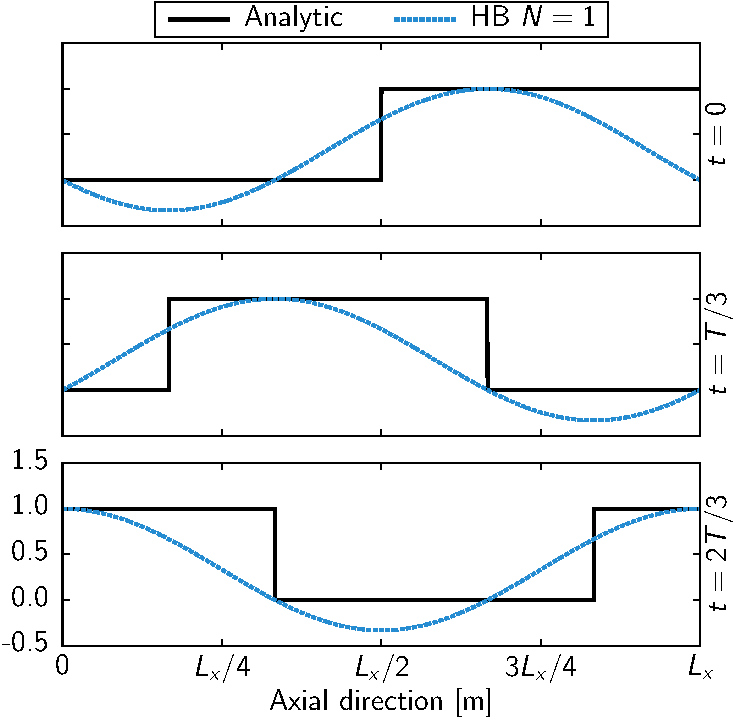
\includegraphics[width=.35\textwidth]{convection_step_N1.pdf}}
  \subfigure[$N=2$]{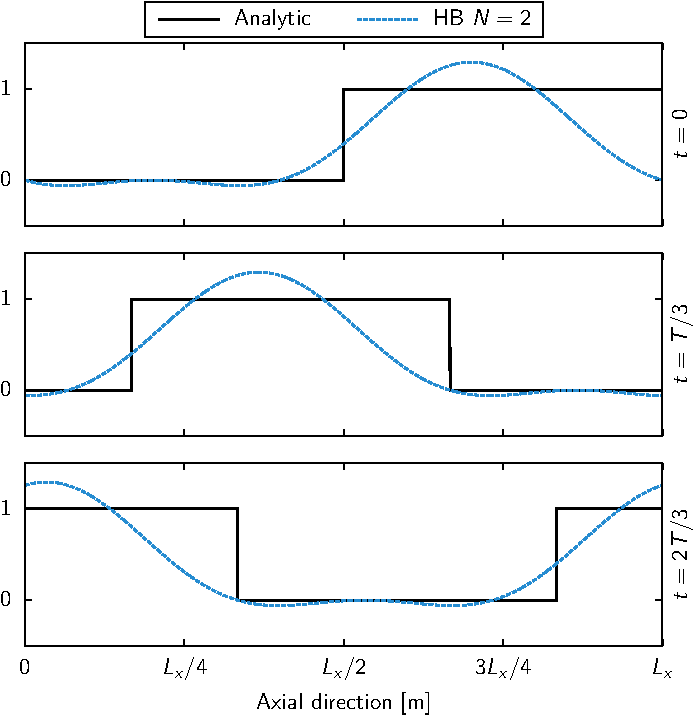
\includegraphics[width=.35\textwidth]{convection_step_N2.pdf}}
  \subfigure[$N=3$]{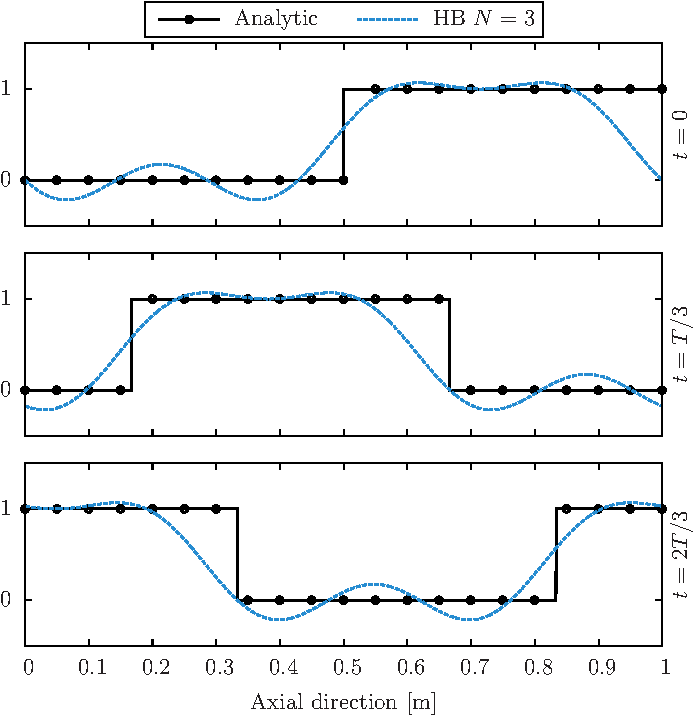
\includegraphics[width=.35\textwidth]{convection_step_N3.pdf}}
  \subfigure[$N=4$]{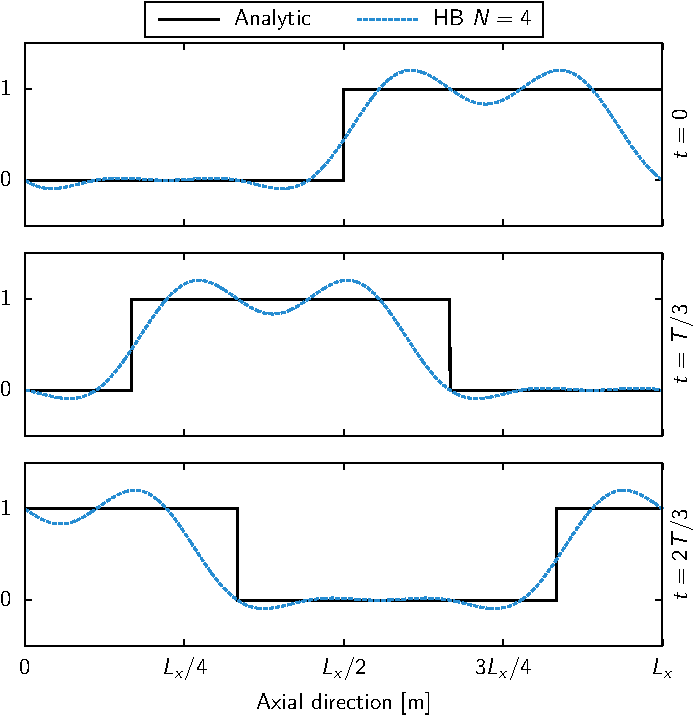
\includegraphics[width=.35\textwidth]{convection_step_N4.pdf}}
  \subfigure[$N=5$]{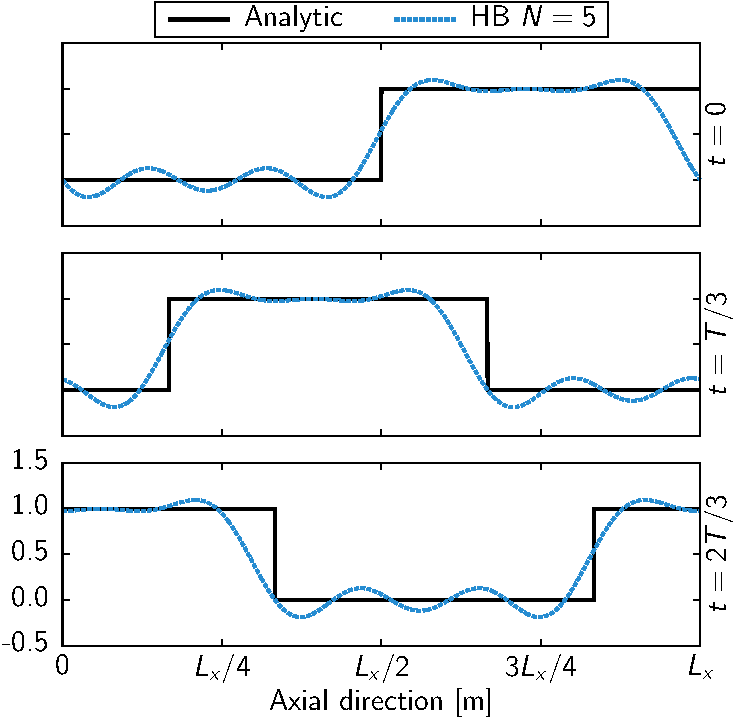
\includegraphics[width=.35\textwidth]{convection_step_N5.pdf}}
  \subfigure[$N=6$]{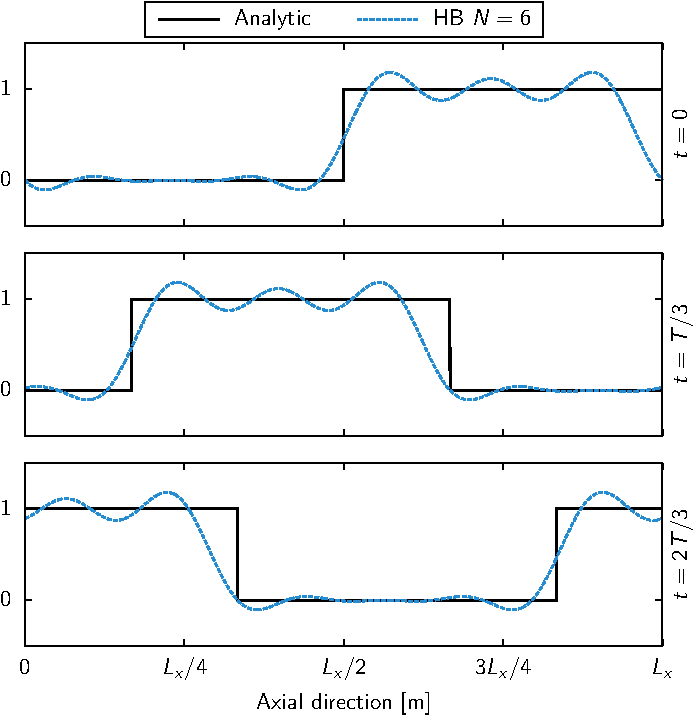
\includegraphics[width=.35\textwidth]{convection_step_N6.pdf}}
  \caption{Linear advection of a rectangular function: 
  numerical solutions at different time instances for different numbers of harmonics.}
  \label{fig:inj_step_results}
\end{figure}
Figure~\ref{fig:inj_step_results} depicts the results of HB computations
using one to six harmonics at different time instances. The convergence rate 
is slow, and for the six-harmonics HB computation the
shape of the rectangular function is still barely captured. 
The well-known \citet{Gibbs1899}
phenomenon is observed, which is a typical drawback 
of Fourier-based methods applied to discontinuous problems, 
see \emph{e.g.} \citet{Canuto2006}.

\begin{figure}[htp]
  \centering
  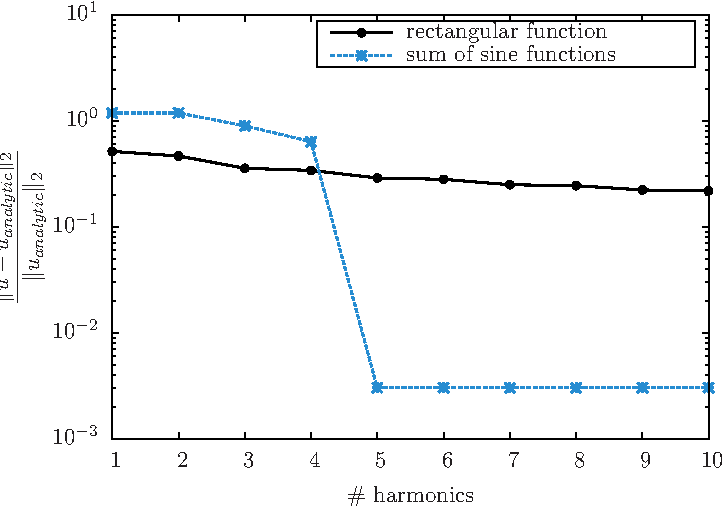
\includegraphics[width=.5\textwidth]{convection_step_error.pdf}
  \caption{Linear advection of a rectangular function: convergence of the HB method error.}
  \label{fig:conv_step}
\end{figure}
The $\mathcal{L}_2$-norm 
of the error is depicted in Figure~\ref{fig:conv_step}. 
The convergence of the sum of sine functions, 
that has been studied in Sec.~\ref{sec:sum_sine},
is added for comparison.
The convergence rate is different from the previous one: 
the error decreases slowly when more harmonics are introduced, 
but the exact solution is never reached, 
unless an infinite number of harmonics is considered.

\begin{figure}[htp]
  \centering
  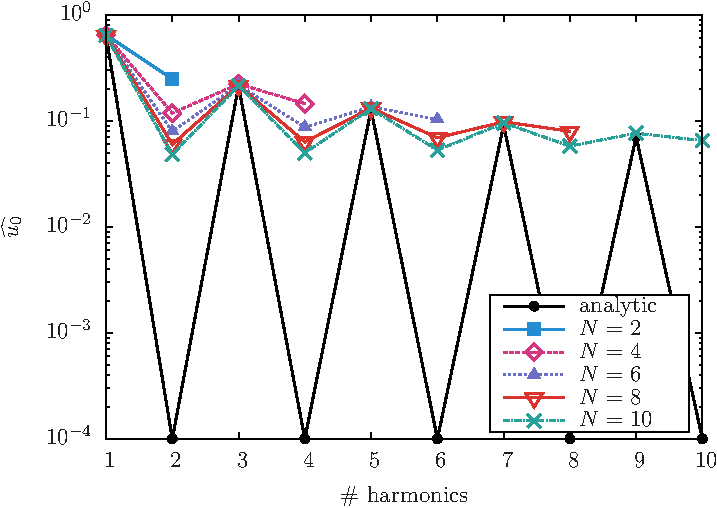
\includegraphics[width=.5\textwidth]{convection_step_dft.pdf}
  \caption{Linear advection of a rectangular function: 
  discrete Fourier transform.}
  \label{fig:dft_step}
\end{figure}
The discrete Fourier transform of the results
is computed and compared to the analytical result in Figure~\ref{fig:dft_step}.
For this case, the spectrum is not finite and cannot be captured accurately
with a finite number of samples.
Adding more harmonics improves the results but the analytical
solution is out of reach of the harmonic
balance approach. 

To summarize, Fourier-based time methods are unadapted
for unsteady signals for which the Fourier spectrum is wide.
In the next section, wake passing is modeled by an analytical
function. This allows to assess the convergence of Fourier-based time
methods for such problems.


\section{Toward turbomachinery wakes}
\label{sec:wake_fct}
%!TEX root = ../../../adrien_gomar_phd.tex

Consider for simplicity a turbomachinery stage composed of two rotors,
as for instance a CROR configuration.
A wake is shed behind the upstream rotor. 
It is stationary in the frame of reference attached to the upstream rotor.
\begin{figure}[htp]
    \centering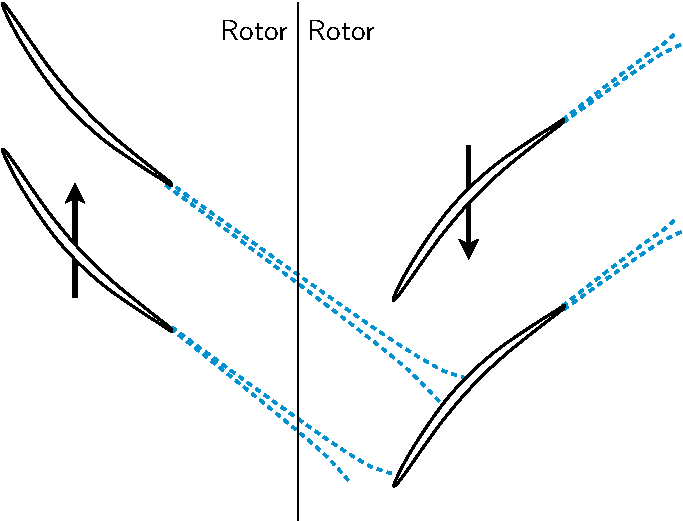
\includegraphics[width=.35\textwidth]{cror_wakes.pdf}
  \caption{Characteristic wakes in a CROR configuration.}
  \label{fig:rotor-stator}
\end{figure}
However, when it crosses the rotor/rotor interface,
the wake becomes unsteady in the frame of reference of the second wheel. 
Thus, an upstream steady spatial distortion becomes unsteady in
the downstream row.

\citet{Lakshminarayana1980} showed that the wake
behind turbomachinery blades follows a similarity law for the velocity. 
It can be empirically approximated by a Gaussian function:
\begin{equation}
    u_l (t) = u_m \left[1 - 
        \Delta u \cdot e^{
          -0.693 \left(2 \frac{\theta}{L} \right) ^ 2}\right],
    \label{eq:similarity}
\end{equation}
where $u_m$ denotes the free-stream velocity, 
$\Delta u$ the axial wake velocity deficit,
and $L$ the wake width,
defined as the full width at half maximum.
The azimuthal coordinate $\theta$ is here assimilated as $c t / L_x$.

Therefore, in the downstream frame of reference, wakes coming 
from the upstream wheel can be represented, 
to a first approximation, as the periodic 
advection of a Gaussian function from the inter-wheel interface.

To study the convergence properties of such a function,
we consider again the linear advection problem defined in Sec.~\ref{sec:linear}, 
with $u_l$ now taken equal to a Gaussian function.
The full width at half maximum $L$ of the wake is set to 10\% of the domain size, 
$u_m$ is set to $c$ and $\Delta u$ to 10\% of $u_m$.

\begin{figure}[htp]
  \centering
  \subfigure[$N=1$]{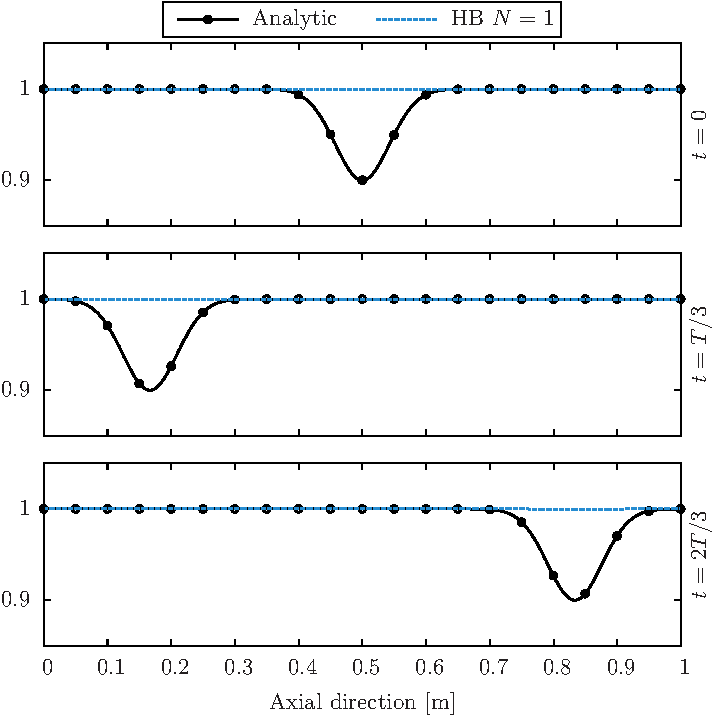
\includegraphics[width=.35\textwidth]{convection_wake_N1.pdf}}
  \subfigure[$N=2$]{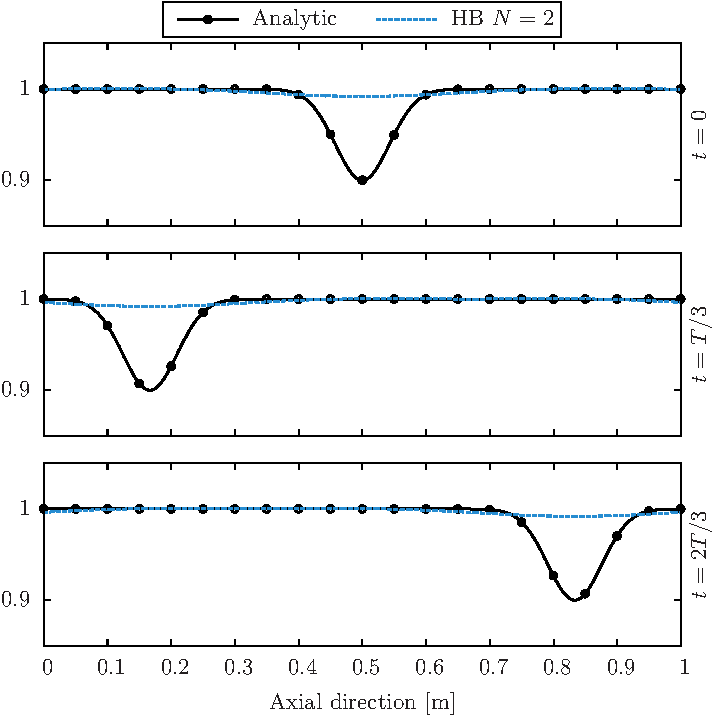
\includegraphics[width=.35\textwidth]{convection_wake_N2.pdf}}
  \subfigure[$N=3$]{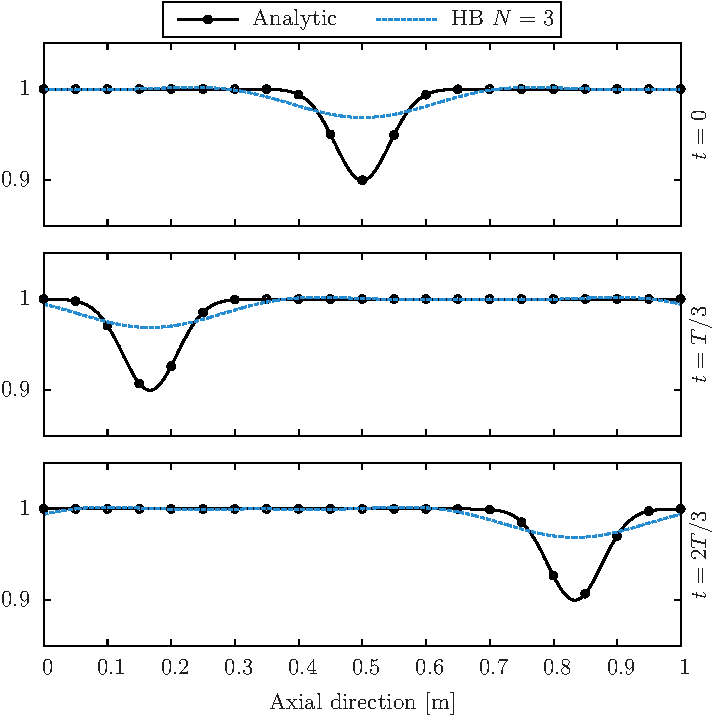
\includegraphics[width=.35\textwidth]{convection_wake_N3.pdf}}
  \subfigure[$N=4$]{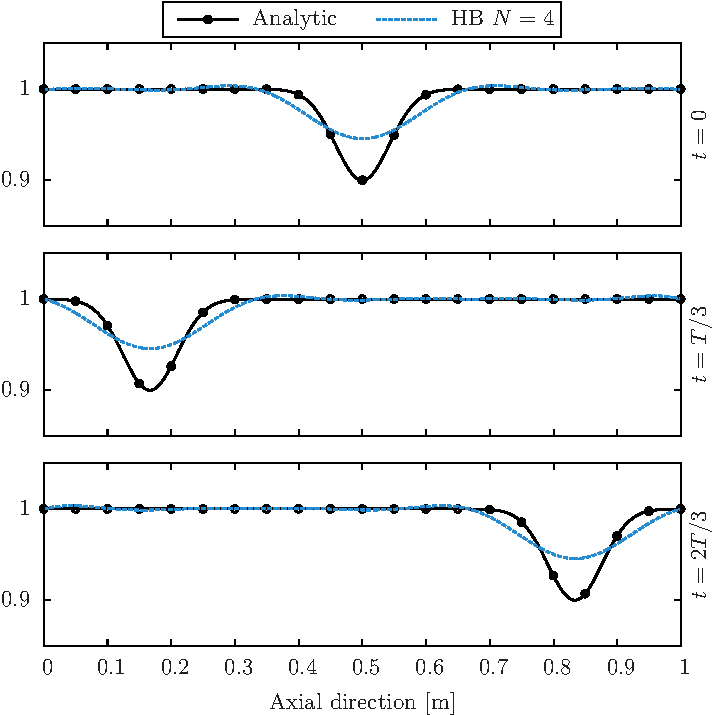
\includegraphics[width=.35\textwidth]{convection_wake_N4.pdf}}
  \subfigure[$N=5$]{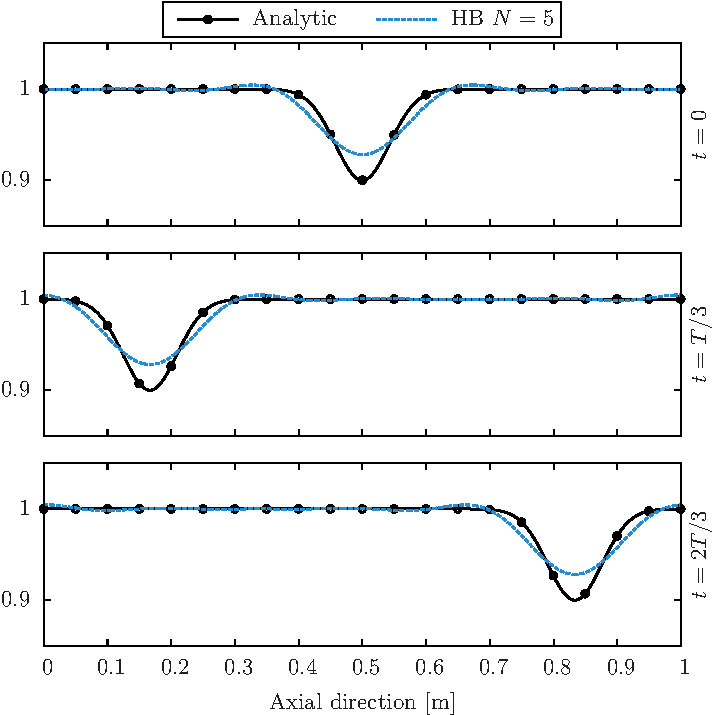
\includegraphics[width=.35\textwidth]{convection_wake_N5.pdf}}
  \subfigure[$N=6$]{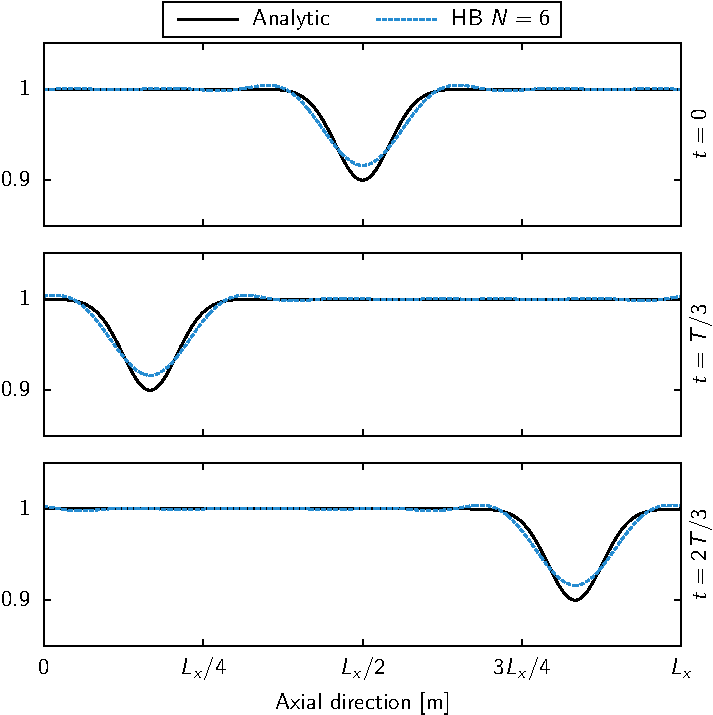
\includegraphics[width=.35\textwidth]{convection_wake_N6.pdf}}
  \caption{Linear advection of a Gaussian function representing a turbomachinery wake: 
  numerical solutions at different time instances for different numbers of harmonics.}
  \label{fig:inj_wake_results}
\end{figure}
Figure~\ref{fig:inj_wake_results} depicts the HB
computations for one to six harmonics. The numerical solution start to convergence
toward the Gaussian function starting from $N=6$ harmonics.
When the number of harmonics is
too small, the width and the depth of the wake are badly approximated
by the method, and the solution exhibits some spurious oscillations. 

\begin{figure}[htp]
  \centering
  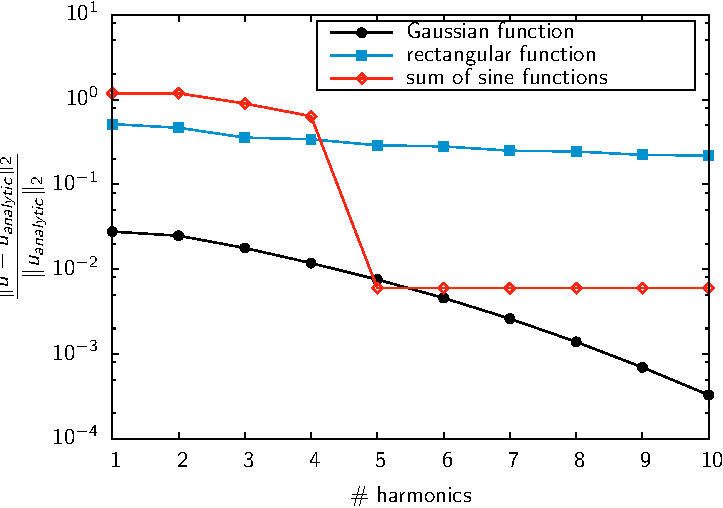
\includegraphics[width=.5\textwidth]{convection_wake_error.pdf}
  \caption{Linear advection of a Gaussian function representing a 
  turbomachinery wake: convergence of the HB method error.}
  \label{fig:conv_wake}
\end{figure}
Figure~\ref{fig:conv_wake} shows the quantitative convergence of 
the $\mathcal{L}_2$ error. The
convergence curves for the two functions studied in the previous sections
are also reported for comparison.
The error follows now a nearly exponential convergence.
\begin{figure}[htp]
  \centering
  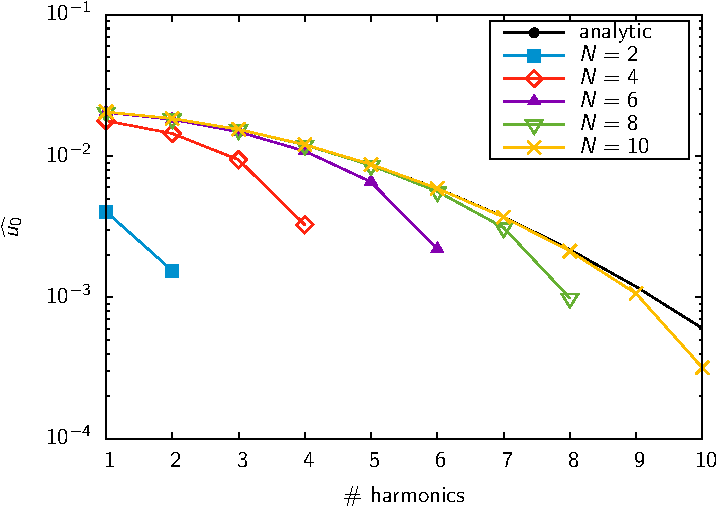
\includegraphics[width=.5\textwidth]{convection_wake_dft.pdf}
  \caption{Linear advection of a Gaussian function representing a turbomachinery wake: 
  discrete Fourier transform.}
  \label{fig:dft_wake}
\end{figure}
The discrete Fourier transform of the results is
depicted against the analytical result in Figure~\ref{fig:dft_wake}.
The $N=2$ and $N=4$ computations badly capture the amplitudes of the
resolved harmonics.
Starting from $N=6$, some of the lower 
frequencies are correctly captured, whereas high frequencies are
always under-estimated.
The capture of the amplitudes 
improves when further harmonics are added to the computation.

For a better understanding of the HB convergence behavior, 
we consider the spectral content of the Gaussian wake model. 
Precisely, the Fourier transform $\widehat{g}$ of a Gaussian function $g$
defined as
\begin{equation}
    g(x) = A e^{-\alpha x^2},
    \label{eq:simple_gaussian_function}
\end{equation}
where $A$ and $\alpha$ are constants, is
\begin{equation}
    \widehat{g}(f) = A^\prime e^{-\alpha^\prime f^2},
    \label{eq:fourier_transform_gaussian}
\end{equation}
where
\begin{equation}
  \begin{cases}
    A^\prime=A \sqrt{\frac{\pi}{\alpha}},\\
    \alpha^\prime = \frac{\pi^2}{\alpha}.
  \end{cases}
\end{equation}
For the similarity law of Lakshminarayana and Davino, 
$\alpha$ and $\alpha^\prime$ can be identified as
\begin{equation}
    \alpha =  0.693 \left( \frac{2}{L} \right)^2, \quad
    \alpha^\prime =  \frac{1}{0.693} \left( \frac{\pi L}{2} \right)^2.
    \label{eq:gaussian_params_laksh}
\end{equation}
The exponential factor of the wake law~$\alpha$ is inversely
proportional to its Fourier counter-part~$\alpha'$, meaning that their
width will vary in opposite way: the thinner the wake, the wider its
spectrum and \emph{vice-versa}.

The convergence rate is inherently linked to
the spectrum of the considered unsteady signal.
As for the present case we know the analytical wake spectrum,
we define the theoretical truncation error as the ratio of
the energy contained in the unresolved part 
of the spectrum to the overall energy content of the full spectrum
\begin{equation}
    \varepsilon_{th}(f) = \sqrt{\frac{
        \int_f^\infty | \widehat{g}(\zeta)|^2 \diff \zeta
      }{
        \int_0^\infty | \widehat{g}(\zeta)|^2 \diff \zeta
      }}.
    \label{eq:def_truncation_error}
\end{equation}
Introducing the error function defined as
\begin{equation}
    \erf(x) = \frac{2}{\sqrt{\pi}} \int_0^x e^{-t^2} \diff t,
\end{equation}
and the complementary error function defined as
\begin{equation}
    \erfc(x) = 1 - \erf(x),
\end{equation}
then
\begin{align}
    \int_0^\infty | \widehat{g}(\zeta)|^2 \diff \zeta 
    &= \frac{1}{2} \int_{- \infty}^\infty | \widehat{g}(\zeta)|^2 \diff \zeta \\
    &= \frac{A^{\prime 2}}{2} \sqrt{\frac{\pi}{2 \alpha^\prime}},
\end{align}
and
\begin{equation}
    \int_f^\infty | \widehat{g}(\zeta)|^2 \diff \zeta = 
      \frac{A^{\prime 2}}{2} \sqrt{\frac{\pi}{2 \alpha^\prime}} \erfc (\sqrt{2 \alpha^\prime} f).
\end{equation}
The theoretical truncation error can finally be written as
\begin{equation}
    \varepsilon_{th}(f, L) = \sqrt{\erfc (\sqrt{2 \alpha^\prime(L) } f)}.
    \label{eq:analytical_conv}
\end{equation}
One can notice from Eq.~\eqref{eq:analytical_conv} that the 
truncation error does not depend on the wake deficit $\Delta u$ 
but only on the wake width $L$.

\begin{figure}[htp]
    \centering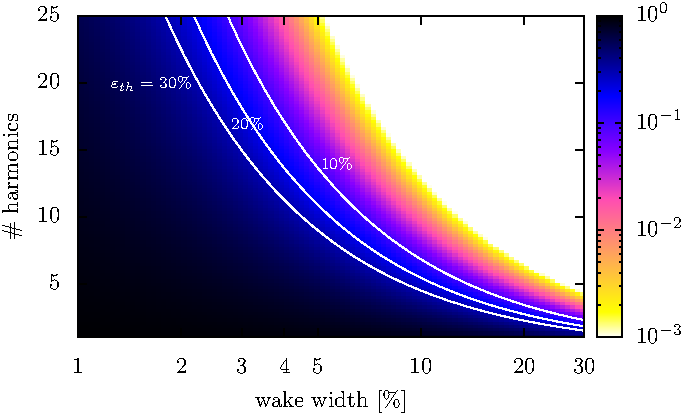
\includegraphics[width=.5\textwidth]{ANALYTICAL_ERROR_PPT.pdf}
  \caption{Theoretical truncation error of the Lakshminarayana and Davino wake law.}
  \label{fig:analytic_error_paper}
\end{figure}
Eq.~\eqref{eq:analytical_conv} is depicted in
Figure~\ref{fig:analytic_error_paper} for varying
numbers of harmonics and wake widths.
It can be seen that the wider the spectrum,
the higher the number of harmonics needed to
reach a certain level of error. 
Moreover, for a thin wake width (\emph{e.g.} 2\% of the pitch)
the number of harmonics required to capture it with a truncation 
error of 10\% is up to 25~harmonics.
In the limit of $L \to 0$, the wake becomes a Dirac function
which represents the worst possible case, as the rectangular
function was.
In the preceding example, the Gaussian function had a width
of 10\% which, according to Eq.~\eqref{eq:analytical_conv},
is captured by using $N=7$ harmonics for a target of 10\% error.

This section provided analytical results of the
convergence of Fourier-based time methods 
in the case of wake passing. To confirm these results,
a turbomachinery like model problem
is set up and solved using the Euler equations in
the following section.





\section{Application to a model turbomachinery configuration}
\label{sec:model_tbm}
%!TEX root = ../../../adrien_gomar_phd.tex


\subsection{Extension of the harmonic balance approach to
  turbomachinery computations}
\label{sec:turbomachinery_adaptation}

To efficiently apply the HB approach to turbomachinery
configurations, phase-lag boundary conditions~\cite{Erdos1977} are
used to cut down the mesh size by using a grid that spans only one
blade passage per row. The phase-lag boundary conditions are two-fold:
i) the azimuthal boundaries of a passage and ii) the blade row
interface which must handle different row pitches on either
sides. Furthermore, in the HB framework, each row captures the blade
passing frequency of the opposite row leading to different time
samplings solved in each row.

The phase-lag condition is based on the space-time periodicity of the
flow variables. It states that the flow in one passage~$\theta$ is the
same as the next passage~$\theta+\Delta\theta$ but at another
time~$t+\delta t$:
\begin{equation}
  W\left(\theta+\Delta\theta,t \right) = W\left(\theta,t+\delta t \right),
  \label{eq:choro}
\end{equation}
where $\Delta \theta$ is the pitch of the considered row.  The time
lag $\delta t$ can be expressed as the phase of a rotating wave
traveling at the same speed as the relative rotation speed of the
opposite row: $\delta t=\beta/\omega_\beta$.  The Inter-Blade Phase
Angle $\beta$ (IBPA) depends on each row blade count and relative
rotation speed. It is analytically given \citet{Gerolymos1991}.  The Fourier
transform of Eq.~\eqref{eq:choro} implies that the spectrum of the
flow in a passage is equal to the spectrum of the neighbor passage
modulated by a complex exponential depending on the IBPA:
\begin{equation*}
%  \label{eq:serfourphasetemps}
  \widehat{W}_k(x, r,  \theta+\theta_G)  = {\widehat{W}_k(x, r,
    \theta)e^{i k\beta}}.
\end{equation*}
At the azimuthal boundaries, this modulation can be computed on the fly
in the HB framework as a sampling of the time period is always known
and it is straightforward to derive an analytic derivation in the time
domain (see Ref.~\cite{JSicot2012}). The blade row interface is more complex
as the different pitches and relative motion of the rows require to
duplicate the flow in the azimuthal direction using the phase-lag
periodicity. A time interpolation also occurs to take the
different time samplings into account and a non-abutting mesh
technique is applied as the mesh will unlikely have matching
cells. To remove spurious waves, an over-sampling and a filtering are
performed. 

The time-domain harmonic balance method has been implemented 
by CERFACS in the
\emph{elsA} solver~\cite{Cambier2013} developed by ONERA. 
This code solves the RANS equations using a cell-centered
approach on multi-blocks structured meshes.  Using the HB method,
significant savings in CPU cost have been observed in various
applications such as rotor/stator interactions~\cite{JSicot2012}
and dynamic derivatives computation~\cite{CIHassan2011}. 


\subsection{Spectral convergence study}
The primary interest in this section is the wake capturing capabilities of the 
Fourier-based time method in the rotating part. 
To analyze this, two error measures are defined and
evaluated. 

\subsubsection{Spatial-spectrum based error measure}
\label{sec:crit_1}
Initially, we propose an error measure ($\varepsilon_1$) based 
on the loss of signal energy
induced by the harmonic method at the interface. 
In fact, in the stator part, the wake is steady and is thus not
filtered by the HB operator. 
Conversely, in the rotor part, the steady wake becomes
unsteady due to the relative speed difference between the
stator and the rotor. However, only a finite number of harmonics~$N$
is used to describe the unsteady field, hence the filtering.

The first error quantification is set up to quantify this filtering 
by using only spatial information and is defined as the $\mathcal{L}_2$-norm 
applied on the 
difference between the rotor and the stator spectra.
It is equivalent to the analytical truncation error 
defined in Eq.~\eqref{eq:def_truncation_error}. 
Indeed, the error is described as the ratio of the unresolved energy 
in the rotor block
to the energy of the full spectrum, 
\emph{e.g.} that of the stator block:
\begin{equation}
    \varepsilon_1(N) = \sqrt{
    \frac{\sum_{f=1}^{f_{max}} | \widehat{s}^{~\theta}_N (f) - 
      \widehat{r}^{~\theta}_N (f)|^2}{ 
    \sum_{f=1}^{f_{max}} | \widehat{s}^{~\theta}_N (f)|^2}},
    \label{eq:def_crit_1}
\end{equation} 
where $\widehat{s}^{~\theta}_N$ denotes the spatial Fourier transform (indicated by
the $\widehat{\vphantom{s}.}$ operator) of the azimuthal extraction (shown
by superscript $\theta$) of the result of a HB simulation using $N$~harmonics,
in the stator; $\widehat{r}$ denotes the spectrum of 
the signal transferred to the rotor.
The higher frequency present in the spectrum is dictated 
by the spatial discretization. Thus, $f_{max} = 1 / 2\Delta \theta_{cells}$, 
using the notations of Eq.~\eqref{eq:az_spatial_discretization_1}.
As the azimuthal cell size is similar in both blocks, 
the same sampling is used leading to the same 
frequencies in both stator and rotor spectra.
Details of the algorithm used to compute $\varepsilon_1$ 
are given in \ref{app:epsilon_1_steps}.

The filtering introduced by the HB approach 
acts primarily on the time resolution. 
For under-resolved HB computations, a dissipation error is observed.
This dissipation is not spatially uniform and gives rise to
dispersion errors on the spatial spectrum and to spurious
high-frequencies as shown in 
Fig.~\ref{fig:spatial_crit} for HB computations $N=2$ to $N=10$.
These effects vanish when the HB computations converge
\emph{i.e.} for $N \geq 10$.
Therefore, the spectrum of the unresolved spurious frequencies 
is imposed to have a zero amplitude value to compute
$\varepsilon_1$.
\begin{figure}[htb]
  \centering
  \subfigure[$N=2$]{
  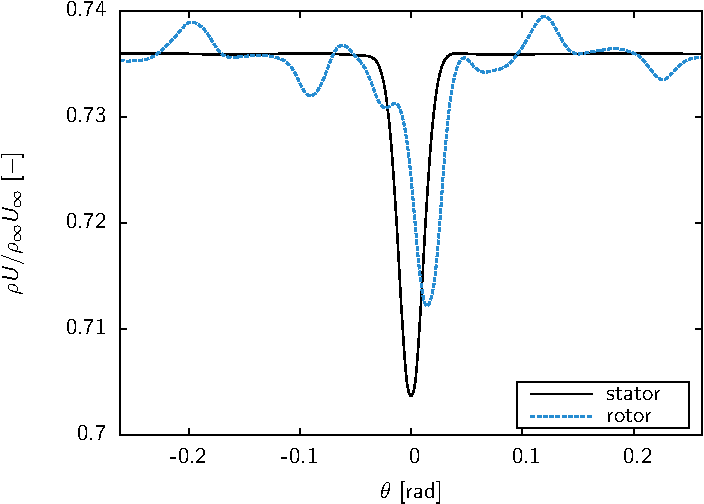
\includegraphics[width=.5\textwidth]{cut_wake_W0490_TSM_N002_adim}
  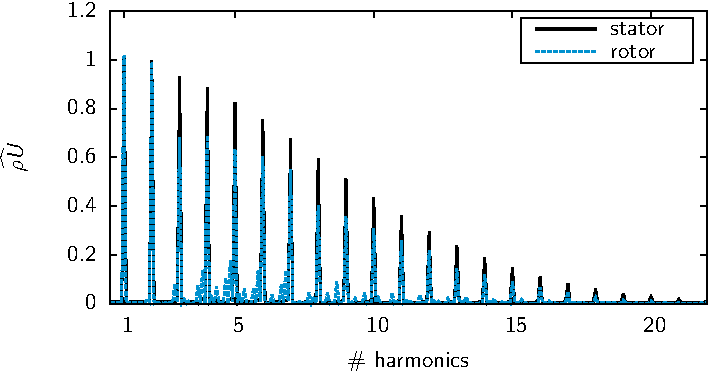
\includegraphics[width=.5\textwidth]{fft_fwake_1D_e490_N02}}
  \subfigure[$N=5$]{
  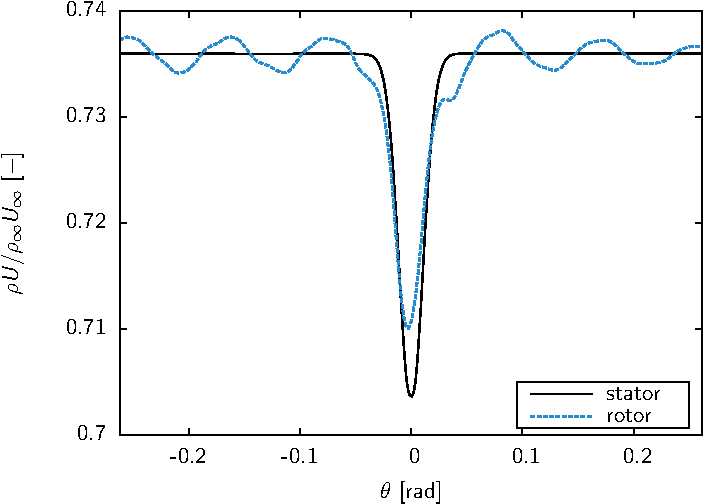
\includegraphics[width=.5\textwidth]{cut_wake_W0490_TSM_N005_adim}
  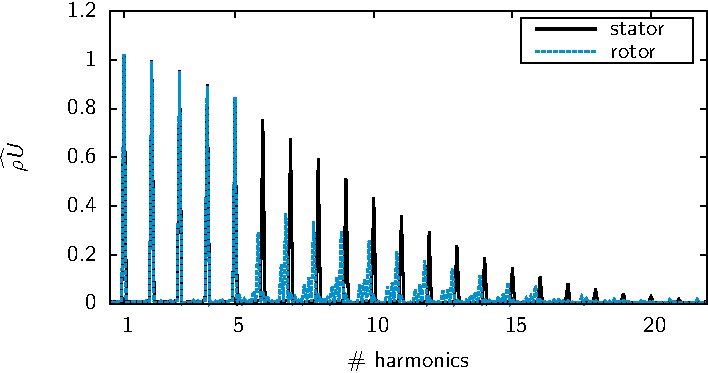
\includegraphics[width=.5\textwidth]{fft_fwake_1D_e490_N05}}
  \subfigure[$N=10$]{
  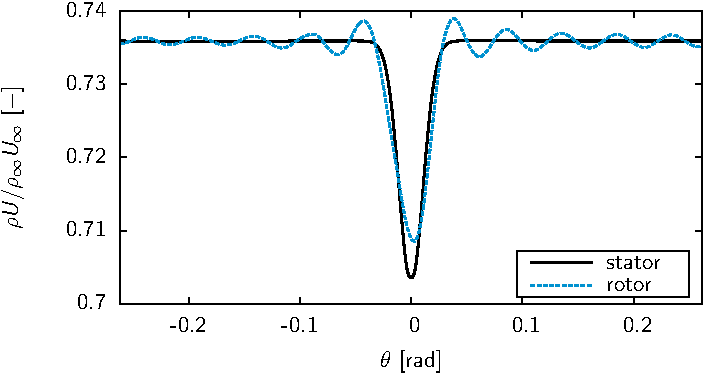
\includegraphics[width=.5\textwidth]{cut_wake_W0490_TSM_N010_adim}
  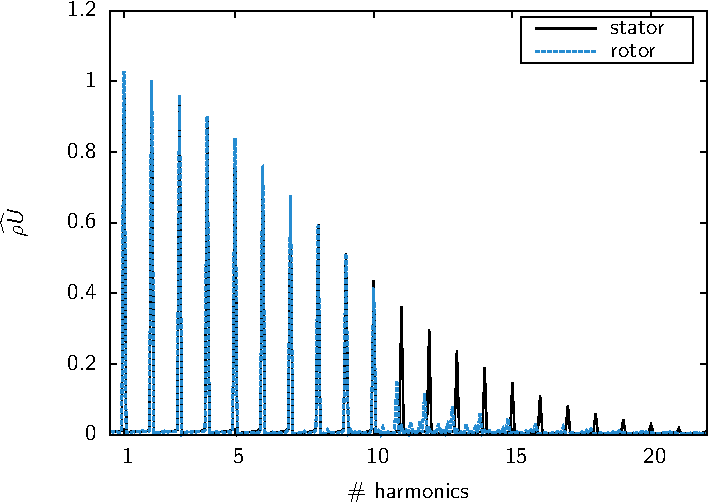
\includegraphics[width=.5\textwidth]{fft_fwake_1D_e490_N10}}
  \subfigure[$N=20$]{
  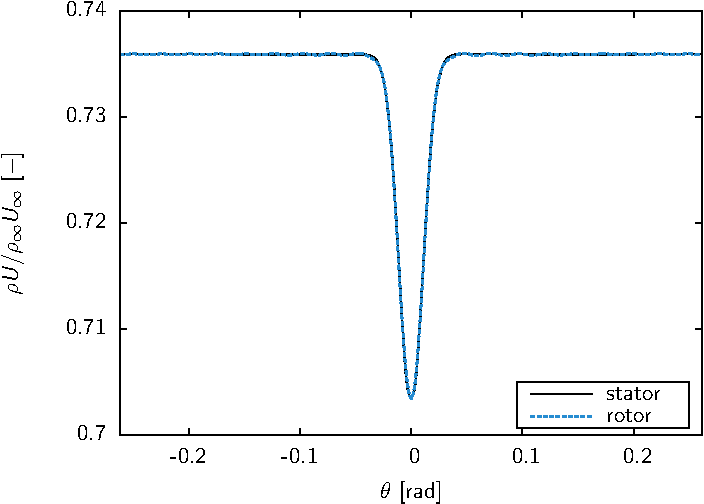
\includegraphics[width=.5\textwidth]{cut_wake_W0490_TSM_N020_adim}
  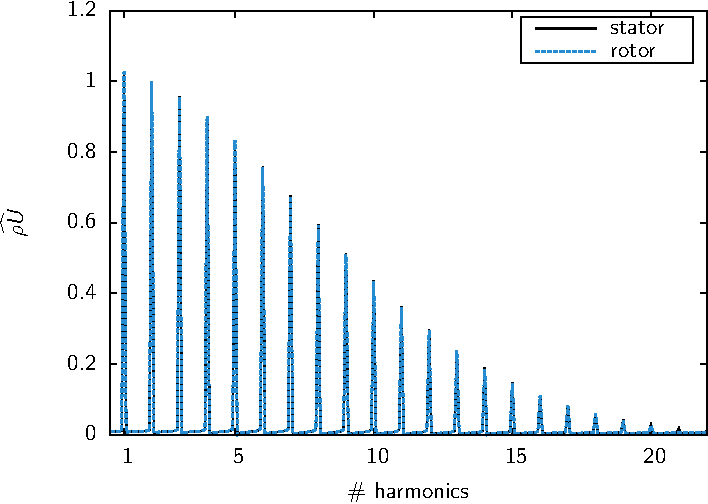
\includegraphics[width=.5\textwidth]{fft_fwake_1D_e490_N20}}
  \caption{Wake of $L=5\%$ width extracted in stator and rotor 
  blocks. Signal and spatial Fourier analysis for different computations.}
  \label{fig:spatial_crit}
\end{figure}

The azimuthal velocity distributions (left hand-side) and the corresponding spatial
spectra (right hand-side)
are presented in Fig.~\ref{fig:spatial_crit} 
for a relative wake thickness of~5\% with respect to the pitch 
and for HB computations using $N=2$, 5, 10 and 18, respectively.
For the stator, the azimuthal distribution follows a 
Gaussian function as expected. On the contrary, 
the rotor distribution is aliased by the HB discretization 
and exhibits spurious oscillations that tend to disappear
when the number of harmonics used in the computation 
increases.
For $N=10$, some oscillations are still present, 
but the wake captured in the moving block begins to 
converge to that leaving the upstream block.

Inspection of the spectra suggests the same conclusions.
The amplitude of $\widehat{\rho U}$ 
improves when increasing the number of harmonics.
As previously mentioned, for under-resolved HB computations,
a dispersion error is introduced and spurious high-frequencies appear 
in the spatial spectra as shown in Fig.~\ref{fig:spatial_crit}
for $N=2$ to $N=10$.
For $N=20$, the spectrum of the rotor 
block matches that of the stator block.
This is consistent with the theoretical analysis, in which more than 
$N=10$ harmonics are needed to capture the wake with less than $20\%$ 
of error for this particular
wake width (see Fig.~\ref{fig:analytic_error_paper}).

In summary, for this wake thickness, the effective temporal filtering 
on a simulation involving less than ten harmonics is too harsh and leads 
to a significant amount of unresolved energy, 
which deteriorates the numerical representation
of the wake.

For a more quantitative analysis, we compute the error measure
$\varepsilon_1$ for each computation ranging over different 
wake thicknesses and numbers of harmonics. 
Results are summarized in Fig.~\ref{fig:crit_1_3d}.
\begin{figure}[htb]
    \centering\includegraphics[width=.6\textwidth]{epsilon_1}
  \caption{Evaluation of the error due to the wake 
  capturing using the first error quantification $\varepsilon_1$.}
  \label{fig:crit_1_3d}
\end{figure}
As it quantifies the unresolved energy in 
comparison to the resolved energy, $\varepsilon_1$ 
exhibits a behavior similar to that of 
the theoretical error $\varepsilon_{th}$ for a Gaussian function 
(Fig.~\ref{fig:analytic_error_paper}).
The iso-error contours have a similar shape 
as the analytical ones. 
The conclusions are equivalent: the truncation error decreases with 
the wake thickness and with the number of harmonics used to capture the wake.
Nevertheless, for thicker wakes and higher numbers of harmonics, 
the error measure $\varepsilon_1$ is over-estimated. 
For instance, around $N=15$ and for $L=25\%$,
$\varepsilon_1 \approx 10^{-2}$ whereas the theoretical error $\varepsilon_{th}$
is less than $10^{-4}$. The error 
measure $\varepsilon_1$ does not represent a 
realistic measure, because of the spatial 
Fourier transform performed to compute 
the error, as discussed in the following.

As can be seen in Fig.~\ref{fig:ST_discrepancies}, 
the Fourier transform of the spatial signal in the stator block tends to a plateau. 
The thicker the wake, 
the lower the frequency for which the plateau appears: 
approximately 15~harmonics for $L=10\%$
(see Fig.~\ref{fig:ST_discrepancies_a}) and 
6~harmonics for $L=25\%$ (see Fig.~\ref{fig:ST_discrepancies_b}).
Actually, for a $N$-harmonic HB computation, the spectrum is 
explicitly filtered in the moving block leading to an amplitude 
equal to zero above the $N^{th}$ harmonic. 
Therefore, when the HB computations are converged, the difference between the spatial 
spectra in the stator and in the rotor block is driven by the plateau present 
in the spatial spectrum of the stator block.

Although the consequences are observed 
on the lower errors associated with the thickest wakes, 
the constant behavior of the spatial spectrum is 
present on the whole range of wake thickness. 
\begin{figure}[htb]
  \begin{center}
  \subfigure[$L=10\%$, $N=3$]{
    \includegraphics[width=.45\textwidth]{SS_discrep_0965_3_log}\label{fig:ST_discrepancies_a}}
  \subfigure[$L=25\%$, $N=15$]{
    \includegraphics[width=.45\textwidth]{SS_discrep_2400_log}\label{fig:ST_discrepancies_b}}
  \end{center}
  \caption{Discrepancies between spatial and temporal spectra.}
  \label{fig:ST_discrepancies}
\end{figure}

In fact, this behavior is linked to the windowing of the signal on 
a bounded interval, the pitch. To highlight that, the influence of 
a modification on the inlet boundary condition is analyzed.
The inlet wake distortion used in the model turbomachinery configuration is 
originally based on the analytical Lakshminarayana and Davino 
Gaussian law (see Eq.~\eqref{eq:similarity}). However, 
this law is discretized and imposed on a bounded interval 
that spans the angular pitch. As the relative thickness 
increases, the inlet condition diverges from the analytical 
Gaussian law for which the angular pitch is theoretically 
infinite. This is shown in Fig.~\ref{fig:inlet_law_fft} 
through the spectra of three Gaussian laws. The relative 
thickness of the laws are modified through the size 
of the pitch $\Delta \theta$. The multiplication by a factor $100$ 
of the pitch leads to a disappearance of the plateau 
in the spectrum, which accurately matches with the 
Fourier transform of a Gaussian function. 
\begin{figure}[htb]
  \centering
  \subfigure[$\Delta \theta = L$]{\includegraphics[width=.7\textwidth]{inject_pitch_1}}
  \subfigure[$\Delta \theta = 10L$]{\includegraphics[width=.7\textwidth]{inject_pitch_10}}
  \subfigure[$\Delta \theta = 100L$]{\includegraphics[width=.7\textwidth]{inject_pitch_100}}
  \caption{Evolution of the spectrum of the inlet boundary condition for different angular pitch.}
  \label{fig:inlet_law_fft}
\end{figure}

To sum up, a plateau appears in the spatial spectrum of the
stator block. This plateau is explicitly filtered in the
rotor block above the $N^{th}$ harmonic, leading to an over-estimation of the 
first error measure. This over-estimation drives the error value
for higher number of harmonics and thicker wakes.

\subsubsection{Spatial/Time duality error measure}
To get a more realistic error measure, we take 
again into account the energy loss
through the interface, but based on a spatial/time duality. 
As this loss of energy is 
precisely related to the filtering 
introduced on the temporal signal by the HB approach, the second 
error quantification $\varepsilon_2$ addresses the result on 
the temporal information. 

Near the interface of the blocks, consider a fixed observer in
the rotor frame of reference. This observer sees an unsteady 
wake passing as the blocks have a relative speed difference.
The first error quantification has shown the 
influence of the number of harmonics on the spatial signal 
in the rotor block. The error quantification will now
point that this spatial influence is due to a temporal filtering done by
the HB approach.

Following the same notation as in Eq.~\eqref{eq:def_crit_1}, 
the second error measure is written as:
\begin{equation}
    \varepsilon_2(N) = \sqrt{
    \frac{\sum_{f=1}^{f_{max}} | \widehat{s}^{~\theta}_N (f) - 
      \widehat{r}^{~t}_N (f)|^2}{ 
    \sum_{f=1}^{f_{max}} | \widehat{s}^{~\theta}_N (f)|^2}},
    \label{eq:def_crit_2}
\end{equation}
where superscript $t$ denotes the temporal version of
the Fourier transform.
By definition, $\varepsilon_2$
quantifies the matching between a spatial signal
and a temporal information.
Again, the error is described as the unresolved energy 
in the rotor block, 
divided by the energy of the full spectrum, 
e.g. that of the stator block. 
For $\varepsilon_1$, the amplitude 
of the harmonics above the $N^{th}$ one was imposed to zero. 
In contrary, for $\varepsilon_2$, the temporal spectrum 
in the rotor block is, 
by essence null above the $N^{th}$ harmonic, as the filtering 
acts on temporal values. 
Details of the algorithm used to compute $\varepsilon_2$ are given in \ref{app:epsilon_2_steps}.

\begin{figure}[htb]
\centering
  \subfigure[$N=5$]{
  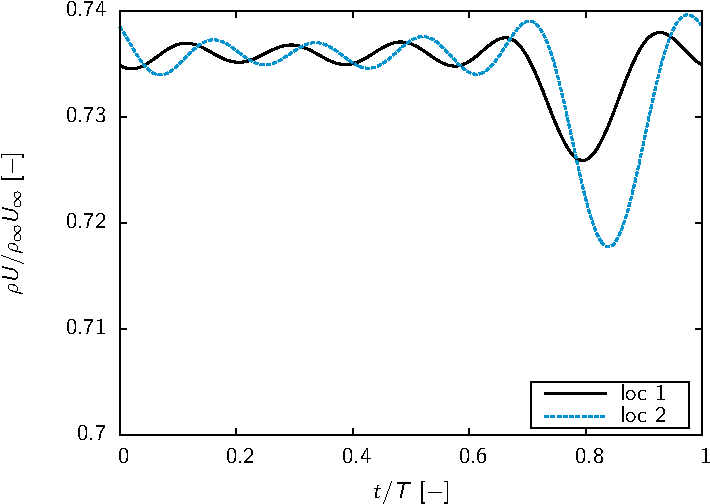
\includegraphics[width=.48\textwidth]{interp_wake_W0490_TSM_N005.eps}
  \label{fig:temp_signal_a}}
  \subfigure[$N=10$]{
  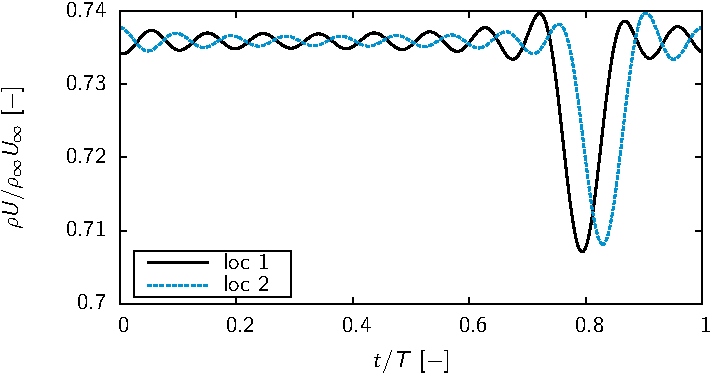
\includegraphics[width=.48\textwidth]{interp_wake_W0490_TSM_N010.eps}}
  \subfigure[$N=15$]{
  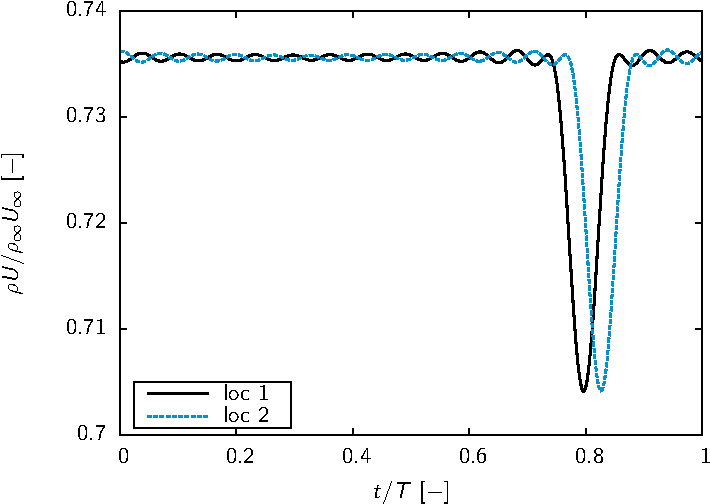
\includegraphics[width=.48\textwidth]{interp_wake_W0490_TSM_N015.eps}
  \label{fig:temp_signal_c}}
  \caption{Temporal signal seen at loc~1 and loc~2 for a $L=5\%$ wake width.}
  \label{fig:temp_signal}
\end{figure}
Figure~\ref{fig:temp_signal} shows time signals
extracted at two different azimuthal positions at 
the interface of the rotor block, named loc~1 and loc~2. 
The small phase shift between the two 
signals is due to the space lag between the two points, 
and is the same for any choice of the number of 
harmonics used in the computation. On the contrary, 
differences in terms of amplitude are only due 
to the use of an insufficient number of harmonics: 
as the number of modes used for the time 
approximation is increased from $N=5$ to $N=15$, 
the amplitude of the space-shifted signals 
tends to converge to the same value, and 
spurious oscillations tend to disappear. Therefore, in the following,
only loc~1 will be considered.

Fig.~\ref{fig:dualite_crit} describes the space and 
time spectra of the axial momentum $\rho U$ at loc~1, 
for computations using $N=2$, 5, $10$ and $20$ 
harmonics and for a wake width of $L=5\%$.
The spatial spectrum contains the whole wavelength 
content associated to the incoming wake; 
on the contrary, due to the filtering introduced 
by the HB approach, the time spectrum is composed of only $N$ harmonics.
\begin{figure}[htb]
\centering
\subfigure[$N=2$]{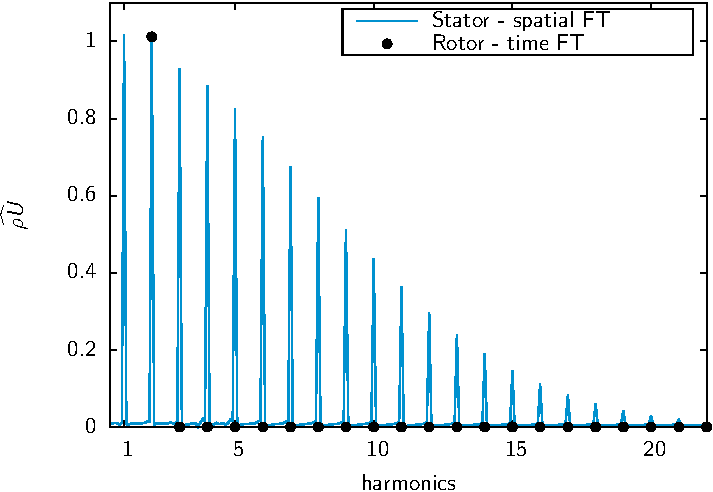
\includegraphics[width=.45\textwidth]{SpcTme_Dualite_0490_02}}
\subfigure[$N=5$]{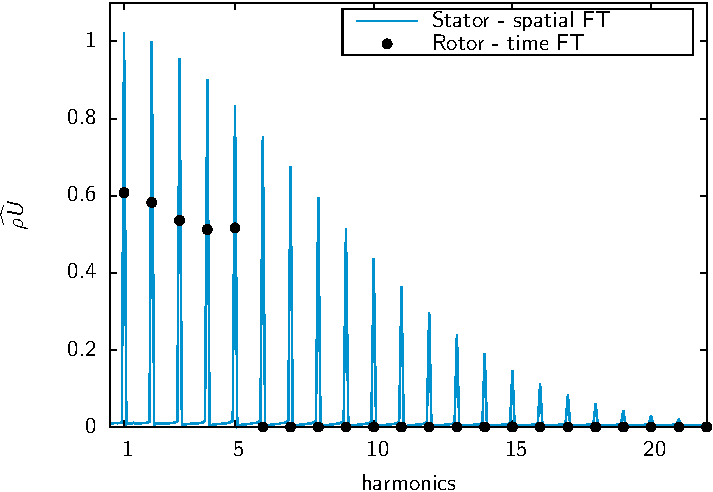
\includegraphics[width=.45\textwidth]{SpcTme_Dualite_0490_05}}
\subfigure[$N=10$]{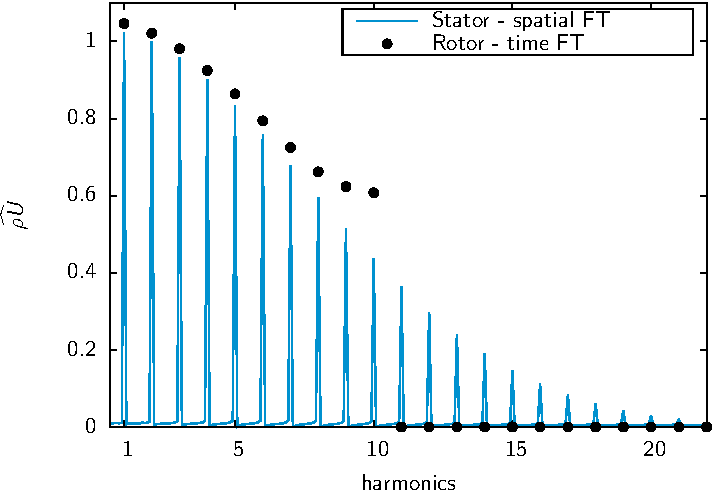
\includegraphics[width=.45\textwidth]{SpcTme_Dualite_0490_10}}
\subfigure[$N=20$]{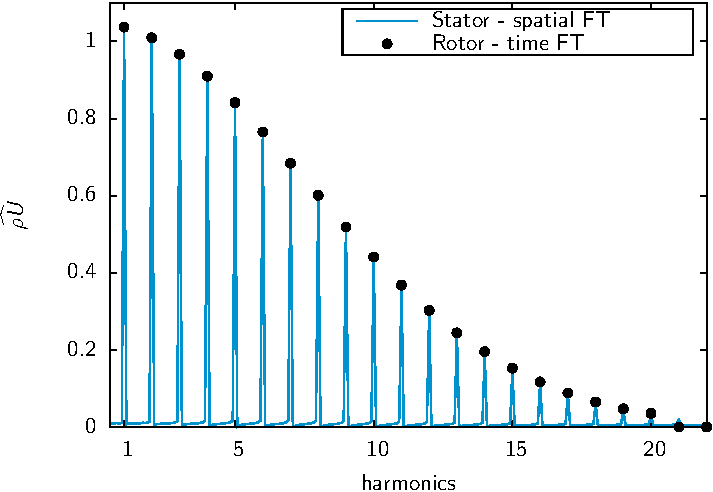
\includegraphics[width=.45\textwidth]{SpcTme_Dualite_0490_20}}
\caption{Spatial/time duality for a $L=5\%$ wake width.}
\label{fig:dualite_crit}
\end{figure}

For computations using less than 10 time harmonics, 
time spectra are truncated, and the amplitude of 
$\rho U$ differs from that of the corresponding mode in the spatial spectrum.

As the number of time harmonics is increased, 
the amplitude of lower harmonics becomes closer 
and closer to that of the corresponding harmonic 
in the reference signal, and errors move toward 
the higher resolved harmonics. For $N=20$, 
the amplitudes of the 20~resolved harmonics are 
similar for both the time and space spectra.

In summary, the preceding analysis shows that, 
for under-resolved HB computations, the time 
signal is affected by both amplitude and phase errors, 
since the energy content is redistributed incorrectly 
among the resolved harmonics.

To quantify this error, we apply the error measure~\eqref{eq:def_crit_2}
to HB computations of the model turbomachinery 
problem corresponding to different choices 
of the wake thickness and different numbers of 
harmonics. Results are presented in Fig.~\ref{fig:crit_2_3d}.
The $\varepsilon_2$ error map is qualitatively 
and quantitatively similar to the $\varepsilon_1$ 
discussed in the previous Section. 
Again, the truncation error measured using $\varepsilon_2$ 
for thick wakes and high numbers of harmonics 
does not follow the trend observed for the 
theoretical error $\varepsilon_{th}$, 
due to the spatial filtering introduced at the 
interface by the phase-lag condition.

The preceding analysis shows that, for HB computations 
that are well converged in terms in harmonics, 
the spatial spectrum in the stator and the 
time spectrum in the rotor block tend to match, 
except for additional spatial errors introduced
by the use of an azimuthal Fourier transform on a 
bounded interval, which confirms the 
validity of the error measure defined in Eq.~\eqref{eq:def_crit_2}.
\begin{figure}[htb]
   \centering \includegraphics[width=.6\textwidth]{epsilon_2_loc_1}
  \caption{Evaluation of the error due to the wake 
  capturing using the second error quantification ($\varepsilon_2$).}
  \label{fig:crit_2_3d}
\end{figure}

\subsection{Comparison with the theoretical error measure}
\label{sub:comp_w_analytic}


The preceding results show that approximated truncation error 
measures computed for the model turbomachinery problem 
using a nonlinear flow model (Euler equations) 
exhibit trends, with respect to the wake thickness 
and number of HB harmonics, in close agreement with the 
theoretical error measure derived in Section~\ref{sec:turbomachine_wake} 
for a Gaussian function. 
Figure~\ref{fig:error_comp_curves} compares the 
different error measures for HB simulations of 
advected wakes of varying thickness versus 
the number of harmonics used for the time discretization. 
This corresponds to horizontal cuts of Figs~\ref{fig:analytic_error_paper}, 
\ref{fig:crit_1_3d} and~\ref{fig:crit_2_3d}. 
For number of harmonics higher than the cutoff 
harmonic used in the phase-lag condition 
the three error measures are seen to give 
results in very close agreement. After that value, 
both the $\varepsilon_1$ and $\varepsilon_2$ error 
measures applied to the model turbomachinery problem 
exhibit a plateau.
The preceding remarks suggest the idea that, 
since all error measure provide similar results, 
at least up to numbers of harmonics of interest for 
practical applicative problems, an a priori 
estimate of the number of harmonics required 
to achieve a given error level could be 
obtained by using the theoretical error measure 
Eq.~\eqref{eq:analytical_conv}, if a quick 
estimate of the wake thickness characteristic 
of a given turbomachinery problem is available. 
In the next Section, we show that a reasonable 
estimate can be obtained from a preliminary steady 
computation based on the mixing plane interface condition.
\begin{figure}[htb]
  \centering
  \subfigure[$L = 2 \%$]{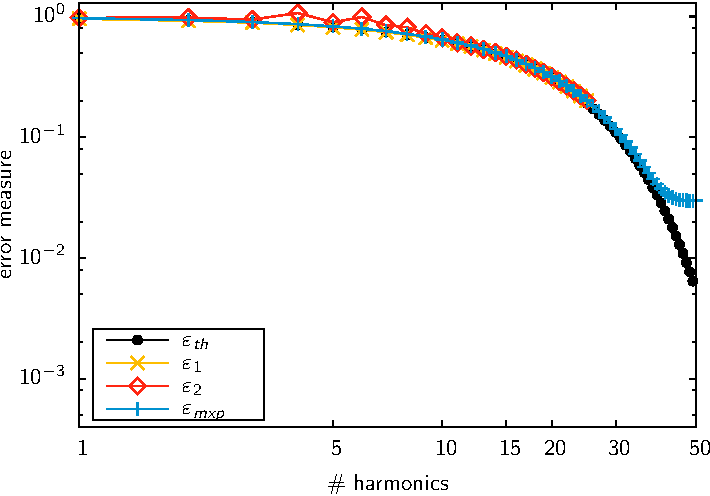
\includegraphics[width=.46\textwidth]{RB_MP_0200_error_logY}}\quad
  \subfigure[$L = 5 \%$]{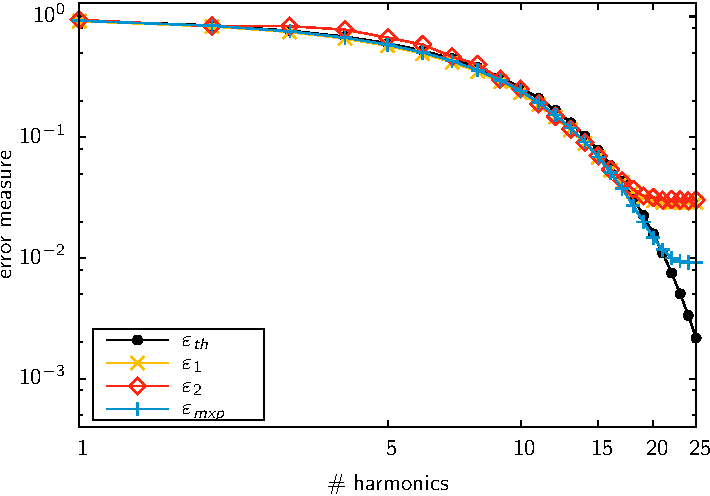
\includegraphics[width=.46\textwidth]{RB_MP_0490_error_logY}}\quad
  \subfigure[$L = 10 \%$]{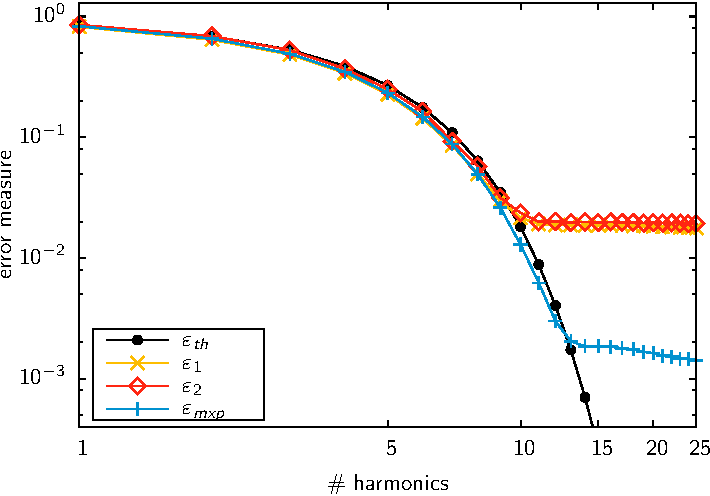
\includegraphics[width=.46\textwidth]{RB_MP_0965_error_logY}}\quad
  \subfigure[$L = 15 \%$]{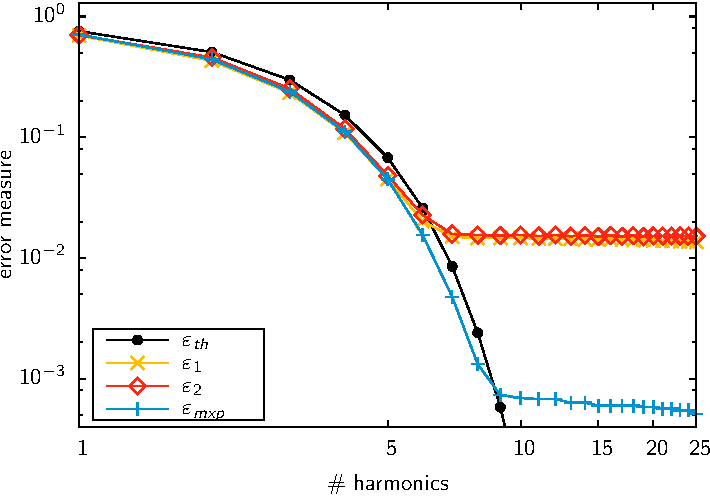
\includegraphics[width=.46\textwidth]{RB_MP_1520_error_logY}}\quad
  \caption{Truncation, computed and analytical errors for four wake width.}
  \label{fig:error_comp_curves}
\end{figure}

\subsection{Toward an priori error estimate}
In order to define an \emph{a priori} error measure 
that can be used to estimate the number of 
harmonics required to achieve a reasonable 
convergence of the HB method, we suggest to 
evaluate the wake thickness by using a preliminary 
mixing plane steady computation. Indeed, if 
potential effects due to the downstream row can 
be neglected, the spatial information at the interface 
in the stator block, essentially due to the incoming 
wakes, can be captured without taking into account 
the relative motion between the wheels, \emph{i.e.} 
by means of a mixing plane computation. 
Given the approximated azimuthal distribution at 
the stator interface, we consider the cumulative
energy content of the signal up to a given frequency $f$ 
(or, equivalently, to a given harmonic $N=f/f_1$ where $f_1$ is the
frequency value of the considered unsteadiness). 
The cumulative energy is defined as:
\begin{equation}
    E(f) = \frac{
      \int_0^f | \widehat{g}(\zeta)|^2 \diff \zeta
    }{
      \int_0^\infty | \widehat{g}(\zeta)|^2 \diff \zeta
    },
\end{equation}
where $\widehat{g}$ is the spectrum of the quantity of interest.
By comparison with Eq.~\eqref{eq:def_truncation_error},
the relation between the relative accumulated energy $E$
and the truncation error $\varepsilon_{mxp}$:
\begin{equation}
    E(f) = 1 - \varepsilon_{mxp}^2 (f).
    \label{eq:correspond_E_error}
\end{equation}


Note that this last error measure is based only on 
the amount of unresolved energy that is left 
in a computation if the spatial signal is 
truncated at a given cutoff frequency $f$, 
and does not require any information from the rotor
block, but it depends only on the characteristics 
of the incoming wake.

To check if the new error measure represents an 
accurate estimate of the truncation error of 
an HB simulation, we carry out again a 
parametric study of the error versus different 
wake thicknesses and numbers of harmonics 
(equivalently, cutoff frequencies), and compare 
the results to those of the \emph{a posteriori} error measures 
obtained for the model turbomachinery problem and for the 
theoretical error $\varepsilon_{th}$. 
Results corresponding to $\varepsilon_{mxp}$ are 
superposed to the corresponding curves in Fig.~\ref{fig:error_comp_curves}. 
The \emph{a priori} error measure ($\varepsilon_{mxp}$) matches 
the theoretical estimate ($\varepsilon_{th}$)
and the \emph{a posteriori} measures ($\varepsilon_1$, $\varepsilon_2$)
over a wide range of harmonics. Similarly to the \emph{a posteriori}
errors $\varepsilon_1$ and $\varepsilon_2$, the \emph{a priori} error
exhibits a plateau for high $N$ and high wake thicknesses, 
due to the application of the Fourier transform on a bounded interval. 
We also stress the close agreement between 
$\varepsilon_{mxp}$ and $\varepsilon_{th}$: specifically, 
estimates of the number of harmonics needed to capture 99\% 
of the cumulative energy (equivalently, to get a 
truncation error equal to 10\%) are identical for 
all error measures.



\chconclu{In this chapter, 
we showed that the main impulsive source of unsteadiness in 
turbomachinery flows is due to the relative motion of wakes 
generated by a given blade row with respect to the downstream row.
\citet{Lakshminarayana1980} showed that the wake shed
behind turbomachinery blades follows a similarity law for the velocity. 
It can be empirically approximated by a Gaussian function.
The Fourier transform of a Gaussian function being analytical,
a truncation error has been defined, which showed that the narrower the wake, 
the larger the Fourier spectrum resulting in a slower convergence 
of Fourier-based time methods.
Based on these observations,
we showed on a model turbomachinery computation, that
the analytical truncation error can be \emph{a priori} 
estimated using a mixing-plane steady computation.
Applying the \emph{a priori} error estimate to 
the steady computation of any turbomachinery configuration
provides a lower bound of the number of harmonics required 
to achieve a given level of convergence.}
